\section{Aufbau und Durchführung}
\label{sec:Durchführung}
\subsection{Versuchsaufbau}
Für den Versuch wird ein Ultraschallechoskop, Ultraschallsonden verschiedener Frequenzen und ein Rechner zur Datenaufnahme und -analyse.
Da das Impuls-Echo-Verfahren genutzt werden soll, wird der Kippschalter am Echoskop auf \textbf{REFLEC.} gestellt. Die Sonden werden an das Echoskop angeschlossen.
Das Programm am Rechner erkennt die Frequenz der Sonden automatisch und zeigt diese an. In der Messsoftware kann nun zwischen einem A- und B-Scan gewählt werden.
Angezeigt wird, je nach Wahl, die Intensität des Signals als Funktion der Messtiefe oder der Laufzeit. Ebenfalls wird die Verstärkung angezeigt, die am Echoskop eingestellt werden kann.
Damit können Intensitätsschwächungen ausgeglichen werden.
Die Messwerte und die angezeigten Graphen können exportiert werden.

\subsection{Durchführung}
\textbf{Untersuchung eines Acrylblocks}\\
\textbf{1. Bestimmung der Abmessungen und Lokalisation der Bohrrungen:}\\
Der Acrylblock wird mithilfe einer Schieblehre vermessen. Dabei wird die Position und die Größe der Bohrrungen bestimmt.\\
\textbf{2. Messung der Laufzeit zur Bestimmung der Schallgeschwindigkeit:}\\
Zur Bestimmung der Schallgeschwindigkeit werden die Laufzeiten für mindestens sieben Löcher gemessen. Mit den zuvor gemessenen Strecken, lässt sich dann 
die Schallgeschwindigkeit berechnen.\\
\textbf{3. Bestimmung der Lage und Größe der Löcher mit einem A-Scan:}\\
Der Acrylblock wird auf ein Tuch gestellt. Mit dem Impuls-Echo Verfahren werden nun die Tiefen aller Löcher gemessen. Es wird von beiden Seiten jeweils eine Messung pro Loch 
durchgeführt. Hierzu ist es ratsam die Intensität als Funktion
der Messtiefe einzustellen. Als Schallgeschwindigkeit $c_{Acryl} = \SI{2730}{m/s}$ in Acryl wird der Literaturwert \cite{acryl} genutzt. Zur Messung wird die 
2MHz Sonde und als Koppelmittel Wasser verwendet.\\
\textbf{4. Bestimmung der Lage und Größe der Löcher mit einem B-Scan:}\\
Die Messsoftware wird auf einen B-Scan umgestellt. Es werden Graphiken von der Unter- und Oberseite aufgenommen und abgespeichert. Zudem werden die Tiefen mithilfe des
Cursors bestimmt und aufgeschrieben.\\
\textbf{Untersuchung des Auflösungsvermögens}\\
Die benachbarten Fehlstellen 1 und 2 in \autoref{fig:block} werden mit der 1MHz und 2MHz Sonde untersucht. Die Graphiken werden bespeichert und sollen ausgewertet werden.\\ 
\textbf{Untersuchung eines Brustmodells mit einem B-Scan:}
Wie in der Theorie beschrieben werden Ultraschallverfahren auch in der Medizin genutzt. In diesem Teil des Versuchs soll mit einem B-Scan ein Brustmodell auf mögliche
Tumore untersucht werden. Ausgenutzt wird dabei, dass Zysten aus einem mit Flüssigkeit gefülltem Hohlraum und Tumore aus einem festen Gewebe bestehen. Das bedeutet, dass
die Intensitäten je nach Tumorart unterschiedlich ist.\\
Zuerst wird das Modell abgetastet. Dann wird ein Koppelgel aufgetragen und das Brustmodell entlang einer Linie untersucht. Das erzeugte Bild wird abgespeichert.
\begin{figure}[H]
    \centering
    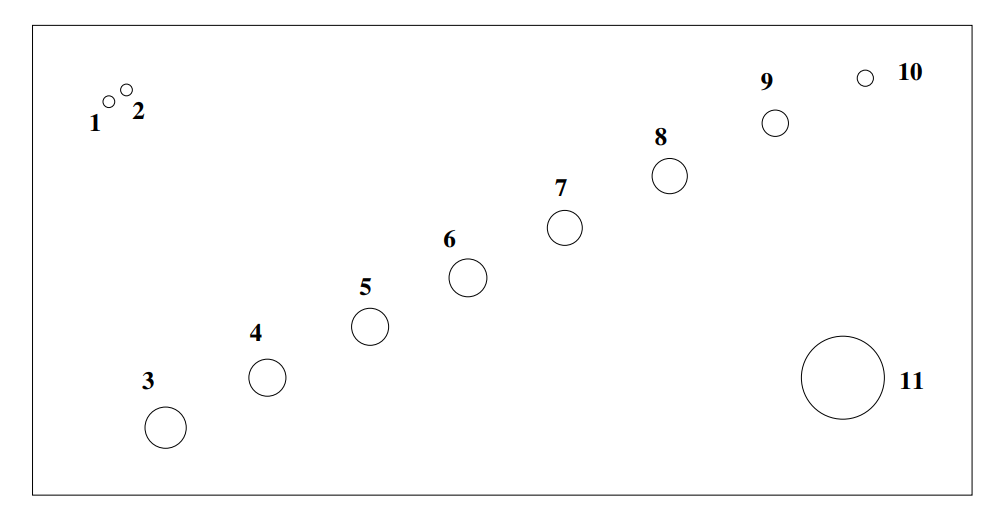
\includegraphics[width=1\textwidth]{img/block.png}
    \caption{Skizze des Acrylblocks \cite{US1}.}
    \label{fig:block}
\end{figure}